実験2は認証機構の追加が通信にどれだけの負荷を与えるのかを
調査するための実験を行った. 
不正ノードの存在しない環境で, 250回シミュレーションを行い, 
遅延時間, パケット配送率, オーバーヘッドサイズを調べた. \\
\indent 実験の結果は以下の通りである. \\

\begin{longtable}{ccc}
  \caption{遅延時間の中央値}
  \label{tab:exp2_delay} \\
  \endfirsthead
  \hline
  \multicolumn{1}{c}{プロトコル} &
  \multicolumn{1}{c}{中央値 [ms]} &
  \multicolumn{1}{c}{最頻値 [ms]} \\ \hline \hline
  No Authentication & $6.88$ & $[6.0, 7.0)$ \\
  DSA & $6.13$ & $[2.0, 3.0)$ \\
  ECDSA & $6.20$ & $[2.0, 3.0)$ \\
  EdDSA & $6.42$ & $[6.0, 7.0)$ \\ \hline
\end{longtable}

\begin{figure}
  \centering
  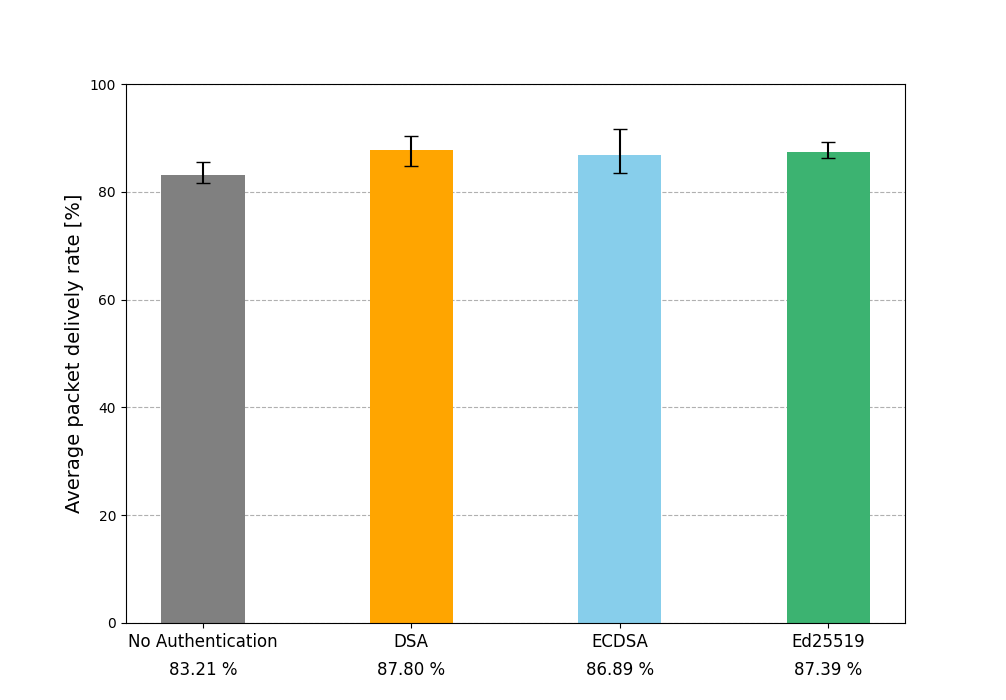
\includegraphics[width=1\textwidth]{figures/exp2_pdr.png}
  \caption{不正ノードが存在しない環境でのパケット配送率}
  \label{fig:exp2_pdr}
\end{figure}
\clearpage
\begin{figure}
  \centering
  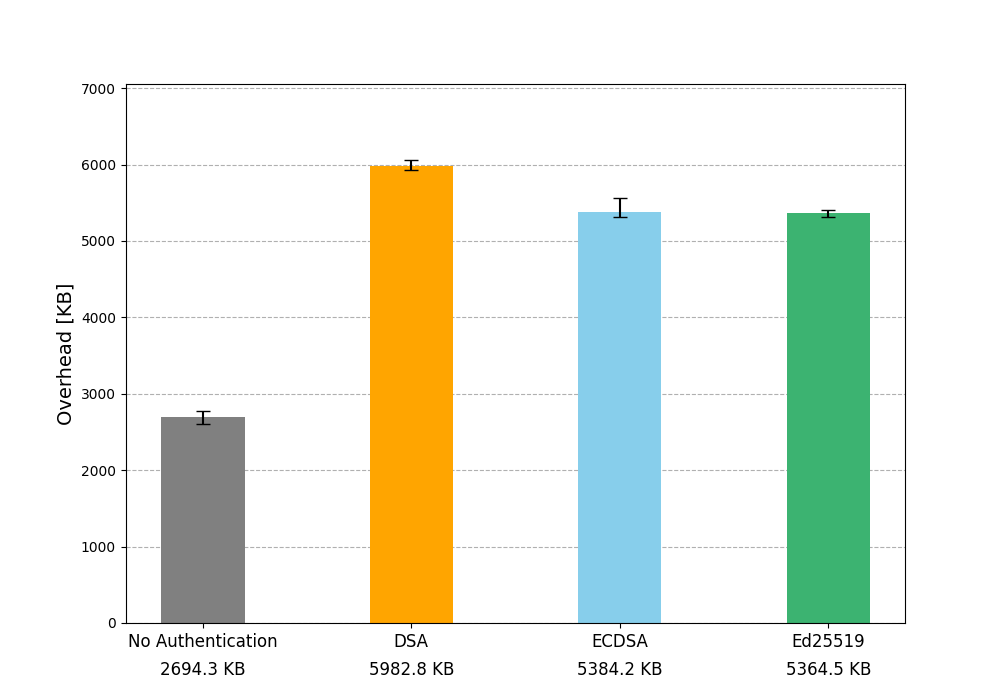
\includegraphics[width=1\textwidth]{figures/exp2_overhead.png}
  \caption{オーバーヘッドサイズ}
  \label{fig:exp2_overhead}
\end{figure}

\indent 表\ref{tab:exp2_delay}は, 実験2におけるシミュレーションパターンごとの
遅延時間の中央値と最頻値を示している. 中央値について, 認証機構なしでは6.88ms, 
DSAでは6.13ms, ECDSAでは6.2ms, EdDSAでは6.42msであった. 
最頻値について, 認証機構なしとEd25519では6.0msから7.0ms, 
DSAとECDSAでは2.0msから3.0msの範囲が最も多かった. 
この結果は, 遅延時間は経路選択のタイミングによって左右されるため, 
若干の差異が出てしまうが, 認証機構の有無が遅延時間に影響を与えなかったことを
示唆している. \\
\indent 図\ref{fig:exp2_pdr}は, 実験2におけるシミュレーションパターンごとの
パケット配送率を示している. 認証機構なしでは83.21 \%, DSAでは87.8 \%, 
ECDSAでは86.89 \%, EdDSAでは87.39 \%となった. この結果から, 
認証機構の有無はパケット配送率に影響を与えなかったと考えられる. \\
\indent 図\ref{fig:exp2_overhead}は, 実験2におけるシミュレーションパターンごとの
オーバーヘッドサイズを示している. 認証機構なしでは
2694.3KBであったのに対し, DSAでは5982.8KB, ECDSAでは5384.2KB, 
EdDSAでは5364.5KBと, 認証機構の追加により
オーバーヘッドサイズが大幅に増加した. これは, Helloパケットの
データに署名が付与されていることが原因である. また, 
EdDSAの結果をDSAとECDSAの結果と比較すると, EdDSAとDSAでは
大きな差があったのに対し, EdDSAとECDSAではほとんど差がなかった. 
EdDSAがDSAよりも鍵長が短いが, ECDSAとは変わらないことから
このような結果になったと考えられる. 
なお, 本研究で使用したパラメータによるそれぞれの鍵長は, 
DSAで2048ビット, ECDSAとEdDSAで256ビットである. \\


